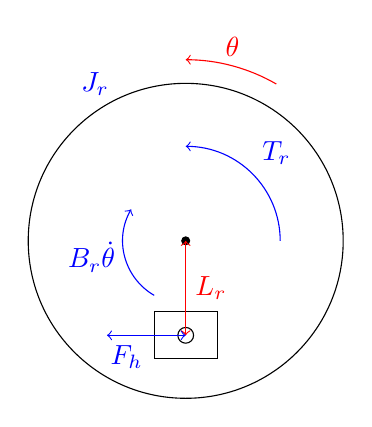
\begin{tikzpicture}
    \draw circle [radius=20mm];
    \draw[fill] circle [radius=0.5mm];
    \begin{scope}[yshift=-12mm]
        \draw circle [radius=1mm];
        \draw (-4mm, -3mm) rectangle (4mm, 3mm);
    \end{scope}
    \draw[<->, red] (0, 0) -- (0, -12mm) node[midway, right] {$L_r$};
    \draw[<->, blue] (0, -12mm) -- +(-10mm, 0) node[near end, below] {$F_h$};
    \draw [->, blue] (-120:8mm) arc (-120:-210:8mm) node[midway, left] {$B_r \dot{\theta}$};
    \draw [->, blue] (0:12mm) arc (0:90:12mm) node[midway, above right] {$T_r$};
    \draw [->, red] (60:23mm) arc (60:90:23mm) node[midway, above] {$\theta$};
    \node[blue] at (120:23mm) {$J_r$};
\end{tikzpicture}
